\section{Distributed Compressed Sensing}
Suppose you are given the task of sensing the spectrum in any given ambient radio environment. At your dispose you have a set of sensors, which have a configurable sampling rate, which you may place anywhere. The only constraint is that no single node is capable of sensing the entire spectrum entirely; however, you are free to decide whether nodes may arrive at consensus (if one can be proven to exist) either in an entirely distributed fashion, or in a coordinated fashion with some node being regarded as centralised, and which does the majority of the data processing.

As we are constrained by the sensing budgets of each node, the data we collect will necessarily be undersampled. However, as discussed in the first chapter, we are capable of designing sensing schemes that are capable of reconstructing signals from undersampled measurements. The trick is designing one which can be distributed over the network, so that we may glimpse the radio environment. 

We do all of this, so that we can make decisions about available transmission opportunities in the spectra. As discussed in Chapter 1 there is a considerable amount of new spectrum being released immanently, and it is being released with the intent that it will be unlicensed. This means that all frequencies in this band (the TV white-spaces) will be available for transmission, without users having to pay for the right to do so. It is hoped that by actively sensing spectral holes, there won't be as many saturated frequencies and that the system will balance itself out. Of course, new users must not interfere with already existing users. 

To achieve our aim of sensing with a set of nodes, we drop our nodes into some geographical area and let the communicate. It's not necessary for every node to talk to every other node. 

Individually the nodes sense a sparse signal, at rates far below the Nyquist rate for that signal, and then collaboratively reconstruct what was sensed. The nodes may all sense the entire signal, or they may sense disjoint portions. In addition, they may sense a signal which is jointly sparse: all the nodes sense a common set of signal components, as well as a set of signal components unique to a particular node. For clarity let \(y_j \in \re^{m_j}\) be the measurement vector obtained by the \(j_{th}\) node, then the measurements can be described by the following linear system:

\begin{equation}
\textbf{y}_j = \textbf{A}_j \textbf{x}_j + \textbf{w}_j
\end{equation}
where \(A_j \in \re^{m_j \times n}\) is a measurement matrix satisfying the restricted isometry property (\ref{RIP}), chosen so that the signal \(x_j \in \re^n\) is suitably sparse (for example, \(A\) could the product of time and frequency representation matrices). \(\vec{w}_j\) is additive white Gaussian noise. 

The matrix is constructed by concatenating the measurements from each sensor, row-wise. That is, we stack the measurements from each node on top of each other.

\subsection{Signal Models}
The core ideas of Distributed Compressed Sensing are to distribute the sensing load among many nodes to reduce the rate required at each node, and to exploit correlations between the data sensed at each node so as to improve the quality of the signals reconstructed at each node. 

The signals at each node are modelled either as having an individual and common part, or as consisting entirely of a common signal. That is,

\begin{equation}
x_j = x_{common} + x_{private,j}
\end{equation}
where \(x_j\) is an \(s\)-sparse signal, and \(x_{common}\) and \(x_{private}\) are \(s_c\)-sparse and \(s_{p_{j}}\)-sparse respectively (\(s_j = s_c + s_p\)) and are assumed to have disjoint support sets.

\subsubsection{Common Signal Model}
This model assumes that all nodes sense the same signal. For example, in wireless telecommunications, all nodes within the same cell would sense a common frequency spectrum. The spectra of distant cells would be independent from each other. Another example could be using sensor networks to monitor seismic activity. 

I.e we have

\begin{equation}
x_j = x_{common} \text{ } \forall j \in J
\end{equation}
note that the sensors may all have different sampling parameters and different noise properties (i.e different SNRs depending on the environment). 

Currently, in this project the common signal model is all that is being considered. 

\subsubsection{Mixed Signal Model}
This is a natural extension of the previous model, allowing for each node to sense individual signal components in addition to the joint component shared by all nodes. The model is,

\begin{equation}
x_j = x_{common} + x_{private,j}
\end{equation}
we recover the previous model by setting \(x_{private} = 0\). This is a slightly more realistic model for spectrum sensing, as it's reasonable to assume that over a cell the signal might not be constant. For example, the joint component might be the signal from a television base-station, whilst the individual signal components may be multipath reflections of other secondary users. 

\subsubsection{Other models}
There are a variety of other models to consider, but all  are some variety of the common plus private paradigm discussed above. For example all nodes could share a common support set for a signal \(x\), however each node may only sense a part of the signal with the full signal being contained in the union of the measurements from all nodes. 

This model can be extended to the common plus private scenario with each node sensing a portion of the joint component in addition to an individual signal component.

It's important to distinguish between distributed models, and distributed solvers. In this sections we have previously described several models in which the sensing is distributed in some way. Now, we proceed to describe several distributed solvers as well as preliminary results of experiments comparing distributed solvers to centralised solvers.

\section{Sensing Model}
\label{sensingmodel}
We are considering a radio environment with a single primary user (PU) and a network of \(J=\)50 nodes collaboratively trying to sense and reconstruct the PU signal, either in a fully distributed manner (by local message passing), or by transmitting measurements to a fusion centre which then solves the linear system. 

\subsection{Setup}
We are trying to sense and reconstruct a wideband signal, divided into \(L\) channels. We have a (connected) network of \(J\) (= 50) nodes placed uniformly at random within the square \(  \left[0,1\right]\times \left[0,1\right] \). They individually take measurements in the following way: by mixing the incoming analogue signal \(x\left(t\right)\) with a mixing function \(p_i\left(t\right)\) aliasing the spectrum. \(x\left(t\right)\) is assumed to be bandlimited and composed of up to \(k\) uncorrelated transmissions over the \(L\) possible narrowband channels - i.e. the signal is \(k\)-sparse. 

This process is repeated in parallel at each node (unrelated to \(N_{sig}\) so that each band in \(x\) appears in baseband. The mixing functions - which are independent for each node - are required to be periodic, with period \(T_p\). Since \(p_i\) is periodic it has Fourier expansion:

\begin{equation}
p_i\left(t\right) = \sum_{l=-\infty}^{\infty} c_{il} \exp\left({jlt\frac{2\pi}{T_p}}\right)
\end{equation}

The \(c_{il}\) are the Fourier coefficients of the expansion and are defined in the standard manner. The result of the mixing procedure in channel \(i\) is therefore \(xp_i\), with Fourier transform:

\begin{align}
X_{i}\left(f\right) &=& \int_{-\infty}^{\infty} x\left(t\right) p_i\left(t\right) dt
\\ &=& \sum_{l=-\infty}^{\infty} c_{il} X\left(f-lf_p\right)
\end{align}

(insert the Fourier series for \(p_i\), then exchange the sum and integral). The output of this mixing process then, is a linear combination of shifted copies of \(X\left(f\right)\), with at most \(\lceil f_NYQ/f_p\rceil\) terms since \(X\left(f\right)\) is zero outside it's support (we have assumed this Nyquist frequency exists, even though we never sample at that rate).

Once the mixing process has been completed the signal in each channel is low-pass filtered and sampled at a rate \(f_s \geq f_p\). In the frequency domain this is a ideal rectangle function, so the output of a single channel is:

\begin{equation}
Y_i\left(e^{j 2 \pi f T_s }\right) = \sum_{l = -L_0}^{+L_0}
\end{equation}

since frequencies outside of \([-f_2/2, f_s/2]\) will filtered out. \(L_0\) is the smallest integer number of non-zero contributions in \(X\left(f\right)\) over \([-f_2/2, f_s/2]\) - at most \(\lceil f_NYQ/f_p\rceil\) if we choose \(f_s = f_p\). These relations can be written in matrix form as:

\begin{equation}
\textbf{y} = \textbf{A}\textbf{x} + \vec{w}
\end{equation}

where \(\textbf{y}\) contains the output of the measurement process, and \(\textbf{A}\) is a product matrix of the mixing functions, their Fourier coefficients, a partial Fourier Matrix, and a matrix of channel co-efficients. \(\textbf{x}\) is the vector of unknown samples of \(x\left(t\right)\). 

i.e. \(\textbf{A}\) can be written: 

\begin{equation}
\textbf{A}^{m\times L} = \textbf{S}^{m\times L} \textbf{F}^{L\times L} \textbf{D}^{L \times L} \textbf{H}^{L \times L}
\label{system}
\end{equation}

The measurements \(\textbf{y}\) are transmitted to a Fusion Centre via a control channel. The system can then be solved by linear programming.

\section{Constrained Convex Optimisation}
We now have a slight diversion into constrained convex optimisation, the denouement of which will not be apparent until later. This section follows (REF), and only contains enough to make the optimisation algorithm on graphs

Say, for example, that you are taking a walk up a mountain and would like to calculate the highest point along your path. You may then be tempted to solve a problem which looked like this:

\begin{equation*}
\begin{aligned}
& \underset{x}{\text{minimize}}
& & f\left( x \right) \\
& \text{subject to}
& & Ax = b
\label{orig_problem}
\end{aligned}
\end{equation*}

where \(f\) is a function in \(\re\), \(A \in \re^{n \times m}\) is a matrix, and \(x\in X\), \(X\) is some convex set.

This is a problem of constrained optimisation, which can be solved by adding a Lagrange multiplier like term to the unconstrained objective (which coincides with the constrained optimisation problem): 

\begin{equation}
L\left(x,y\right) = f\left( x \right) + y^T\left(Ax-b\right)
\end{equation}

where \(y\) is the Lagrange multiplier, and \(L\) is referred to as the Lagrangian. The components of \(y\) can be interpreted as the rate of change of the objective function as a function of the constraint variable. For example, if we are required to find the maximum height along a path on the mountain, the Lagrange multiplier would represent the rate of change in height along that specific path. 

We can find the solution of the original problem via the duality theorem of Fenchel:

\begin{equation}
g\left(y\right) = \inf_x L\left(x,y\right) = -f^*\left(-A^Ty\right) -b^Ty
\label{dual_problem}
\end{equation}

where \(f^*\) is the convex conjugate (Legendre-Fenchel) transform of \(f\). The problem is now to maximise \(g\). 

This maxima can be expressed in closed form as:

\begin{equation}
x^* = \underset{x}{\text{minimize}} L\left(x, y^*\right) 
\label{convex_soln}
\end{equation}

where \(y^*\) is the soln of the dual problem. 

Together \ref{dual_problem} and \ref{convex_soln} suggest a iterative algorithm, which proceeds iteratively by finding a minima of the objective function (up to a convex transformation) and then updating the Lagrange multiplier until some convergence criterion is met: 

\begin{align}
x^{k+1} &:= \underset{x}{\text{minimize}} L\left(x, y^*\right)  \\
y^{k+1} &:= y^{k} + \alpha^k \left(Ax^{k+1} - b\right)
\label{gradient_ascent}
\end{align}

This is a form of gradient ascent, with \( \alpha \) as the step size and \(k\) is the iteration counter. Assuming that \(g\) is differentiable, the algorithm is monotone (i.e. \( g\left(y^{k+1}\right) > g\left(y^{k}\right)\).

This algorithm is easily extended to the case where the objective function is linearly separable. That is scenarios where we can split \(f\left(x\right)\) into a sum of functions \(f_i\left(x_i\right)\), each over a disjoint domain \(x_i \in X_i\) (in our hill walking example, we can split our chosen path into a series of continuous intervals which lay next to each other). Extending the algorithm is simple: all that needs to be done is to perform the minimisation step in (\ref{gradient_ascent}) in each of the functions \(f_i\), and then jointly update the multiplier.

We have assumed the diferentiabilty \(g\) throughout, and it is this smoothness condition which allows the previous algorithm to terminate on a solution of the original constrained problem.

For problems with \(g\) not differentiable, the augmented Lagrangian is introduced as:

\begin{equation}
L_\rho\left(x,y\right) = f\left( x \right) + y^T\left(Ax-b\right) + \frac{\rho}{2}\|Ax-b\|_2^2
\end{equation}

where \(\rho\) is a penalty parameter. That is we're no longer seeking exact solutions, but instead seek solutions close in mean square error. 

The associated dual function is \(g_\rho\left(y\right) = \inf_x L_\rho\). By adding the penalty term, \(g_\rho\) is no differentiable, and the \(\rho \rightarrow 0\) regime corresponds to the solution of the original problem. 

The algorithm in this case can be found by first minimising over \(x\) and then evaluating the resulting equality constraint residual, i.e.:

\begin{align}
x^{k+1} &:= \argmin{x} L_\rho \\
y^{k+1} &:= y^{k} + \rho \left(Ax^{k+1} - b\right)
\label{mom}
\end{align}

This algorithm is known as the method of multipliers for solving the problem (\ref{orig_problem}). Note that even if \(f\) is separable, the augmented Lagrangian may not be.

\subsection{ADMM}
The alternating direction method of multipliers (ADMM), is an algorithm intended to blend the decomposability of the gradient ascent algorithm \ref{gradient_ascent}, with the more general method of multipliers \ref{mom}, i.e. when the objective function is decomposable but the dual function is not differentiable. The algorithm solves problems of the form

\begin{align}
\text{min}_{x} f\left( x \right) + g\left(z\right)
\\
\text{s.t } Ax +Bz = c
\label{admm}
\end{align}

where \(f\) and \(g\) are assumed to be convex function with range in \(\re\), \(A \in \re^{p \times n}\) and \(B\in \re^{p \times m}\) are matrices (not assumed to have full rank), and \(c \in \re^p\). We begin by illustrating a few examples, relevant to the type of problems encountered in signal processing.

\begin{example}
The Basis Pursuit problem

\begin{equation*}
\begin{aligned}
& \underset{x}{\text{minimize}}
& & \|x\|_1 \\
& \text{subject to}
& & Ax = b
\label{bp}
\end{aligned}
\end{equation*}

can be written in the ADMM form (\ref{admm}):

\begin{equation*}
\begin{aligned}
& \underset{x}{\text{minimize}}
& & f\left( x \right) + \|z\|_1 \\
& \text{subject to}
& & x - z = 0
\label{bp_reform}
\end{aligned}
\end{equation*}

where \(f\) is the indicator function of \(\{x\in \re^n : Ax = b\}\). 

\end{example} 

\begin{example}
Similarly the LASSO:

\begin{equation}
\text{minimise } \frac{1}{2}\|Ax-b\|_2^2 + \lambda\|x\|_1
\end{equation}

\(\lambda > 0\), can be solved by the ADMM with \(f = \frac{1}{2}\|Ax-b\|_2^2\) and \(g = \lambda\|x\|_1\).

\end{example}

The solution of (\ref{admm}) is:

\begin{equation}
x* = \inf\{f\left( x \right) + g\left(z\right) : Ax +Bz = c\}
\end{equation}

As previously we form the Lagrangian:

\begin{equation}
L_\rho\left(x,y\right) = f\left( x \right) + g\left(z\right) + y^T\left(Ax+Bz-c\right) + \frac{\rho}{2}\|Ax+Bz-c\|_2^2
\end{equation}

ADMM consists of the iterations:

\begin{align}
x^{k+1} &:= \argmin{x} L_\rho\left(x,z^k,y^k\right)\\
z^{k+1} &:= \argmin{z} L_\rho\left(x^{k+1},z,y^k\right)\\
y^{k+1} &:= y^{k} + \rho \left(Ax^{k+1} + Bz^{k+1} - c\right)
\label{admm_algo}
\end{align}

Note that this algorithm is similar to both the gradient ascent and method of multipliers from the last section: it has an \(x\) minimisation step, an \(z\) minimisation step and a dual variable update. I.e. the Lagrangian is updated simultaneously with respect to the two primal variables. Separating minimisation into two steps (as opposed to joint minimisation) is what allows for decomposition if \(f\) or \(g\) (or both) are separable. 

\section{Constrained Optimisation on Graphs}
We model the network as an undirected graph \(G = \left(V,E\right)\), where \(V = \{1 \ldots J\}\) is the set of vertices, and \(E = V \times V\) is the set of edges. An edge between nodes \(i\) and \(j\) implies that the two nodes can communicate. The number of nodes node \(i\) can communicate is written \(\mathcal{N}_i\) and the degree of node \(i\) is \(D_i = |\mathcal{N}_i|\). 

We assume that a proper (or approximate) colouring of the graph is available: that is each node is assigned a number from a set \(C = \{1 \ldots c \} \), and no node shares a colour with any neighbour.

Given the measurement model from the section (SECTION), we can represent the linear system by concatenating the measurements of each node into a single system. Where, each row of the matrix represents the measurements of a single node. I.e we are trying to solve the following problem:

\begin{equation}
\text{min} ||x||_1 \text{ subject to } A_p x = b_p
\end{equation}

The problem is coupled at each node by the variable \(x\). To ease this issue, at each node create a local copy, denoted \(x_j\) (so there will be \(J\) copies of this variable). 

Then, for consistency, we constrain the problem, so that each copy is identical: \(x_1 = x_2 = \ldots x_J\). Equivalently, given the graphical structure of the problem, we require that \(x_i = x_j\) for each edge of the network.

So now we are solving the problem

\begin{equation}
\text{min} \frac{1}{J}\sum_J||x_j||_1 \text{ subject to } A_p x = b_p \text{ and } x_i = x_j \{i,j\} \in E 
 \label{constrainedbp}
\end{equation}
 
This is exactly the kind of problem that can be attacked by the Alternating Direction Method of Multipliers, described previously. We present a short example for bipartite graphs, which can easily be generalised to graphs with many colours. 
 
\subsection{Example: bipartite graphs}
We are here considering graphs which are connected, and 2-colourable, that is nodes 1 to \(c\) have colour 1 (red say), and nodes \(c+1\) to \(J\) have colour 2 (blue). We will demonstrate that we can decompose problem (\ref{constrainedbp}) into \(c\) problems which can be executed in parallel by minimising \(x\) at the 1st set of nodes, and \(J - c\) problems which also can be executed in parallel by minimising at the second set of nodes. 

Firstly, for compactness, we introduced the arc-incidence matrix of the graph \(B\). This is the \(J \times E\) matrix where each column corresponds to an edge \(\{i,j\} \in E\), with the \(ith\) and \(jth\) entries equal to 1 and -1 respectively. With this notation, we can rewrite (\ref{constrainedbp}) as:

\begin{equation}
\text{min} \frac{1}{J}\sum_J||x_j||_1 \text{ subject to } A_p x = b_p \text{ and } \left(B^T \circ I \right)\bar{x} = 0 
 \label{constrainedbp1}
\end{equation}

where \(\bar{x} = \left(x_1, x_2, \ldots x_J \right)\), and \(\circ\) is the Kronecker product. 

In this form, the Lagrangian of the problem (\ref{constrainedbp1}) can be written in the following way:

\begin{align}
L\left(\bar{x}_1, \bar{x}_2; \lambda\right) = \frac{1}{J}\sum_{j \in C_1}||x_j||_1 + \frac{1}{J}\sum_{j \in C_2}||x_j||_1 &+ \\ \phi_1\left(\bar{x_1}, \lambda\right) + \phi_2\left(\bar{x_2}, \lambda\right) &+ \\
\rho\bar{x}_1^T\left(B_1B_2^T\circ I_n\right)\bar{x}_2
\end{align}
where 

\begin{align}
\phi_i\left(\bar{x}_i, \lambda\right) &= \lambda^T\left(B_i^T\circ I_n\right)\bar{x}_i + \frac{\rho}{2}\vectornorm{\left(B_i^T\circ I_n\right)\bar{x}_i }^2 \\
&= \left(\left(B_i^T\circ I_n\right)\lambda \right)^T\bar{x}_i + \frac{\rho}{2}\bar{x}_i^T\left(B_1B_2^T\circ I_n\right)\bar{x}_i
\end{align}

Since, no nodes within \(C_i\) are neighbours \(B_iB_i^T\) is a diagonal matrix (with the degree of node \(i\) as the \(i\)th entry). So, we can finally re-write

\begin{equation}
\phi_i\left(\bar{x}_i, \lambda\right) = \sum_{j \in C_i}\left(\left(\sum_{k \in \mathcal{N}_i} sign\left(k-i\right)\lambda_{\{i,k\}}\right)^T x_i + \frac{\rho}{2}D_i\vectornorm{x_i}^2  \right)
\end{equation}

where the dual variable \(\lambda\) has been decomposed edge-wise so that \(\lambda_{\{i,j\}} = \lambda_{\{j,i\}}\) and is associated with edge \(\{i,j\}\) and the constraint \(x_i = x_j\).
 

\section{Results and Simulations}
50 nodes were dropped into the square \( \left[0,1\right] \times \left[0,1\right] \), and they make measurements according to the sensing model in section \ref{sensingmodel}. A random 'spike-train' signal was generated: where the spikes were placed uniformly at random in a length 201 vector (representing 201 available channels in a power spectral density of a wideband signal). 

\begin{figure}
\centering
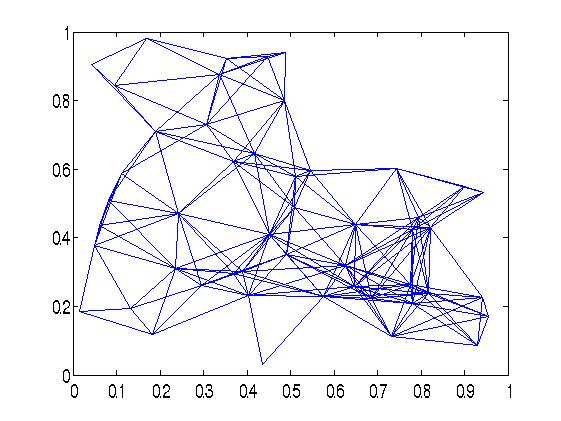
\includegraphics[height = 7 cm]{examplegraph.jpg}
\caption{An example configuration of nodes}
\label{exgraph}
\end{figure}

For a series of SNR values, the system (\ref{system}) was simulated, the mean squared error (mse):

\begin{equation}
\mathbb{E}\left( \frac{\| \hat{x}-x \|}{\| x \|} \right)
\label{mse}
\end{equation}

was calculated for both a centralised (SPG-L1) and decentralised solver (D-ADMM). In the equation above (\ref{mse}) \(\hat{x}\) refers to the estimator of the signal \(x\), found as the solution to the basis pursuit denoise problem:

\begin{equation*}
\begin{aligned}
& \underset{x}{\text{minimize}}
& & \frac{1}{2}\|\hat{x} - Ax\|_2^2 + \lambda\|x\|_1 \\
& 
\label{bpdn}
\end{aligned}
\end{equation*}

The following diagram shows the results of this experiment: 

\begin{figure}
\centering
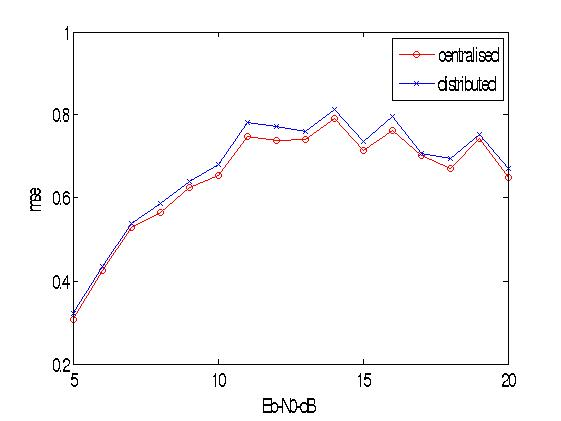
\includegraphics[height = 7 cm]{msevssnr.jpg}
\caption{Mse vs SNR for the sensing model, for distributed and centralised solvers}
\label{msevssnr1}
\end{figure}

This is clearly incorrect: for example it implies that by adding noise you can improve a communication system. The same system was simulated without a graph, and the following result was produced:

\begin{figure}
\centering
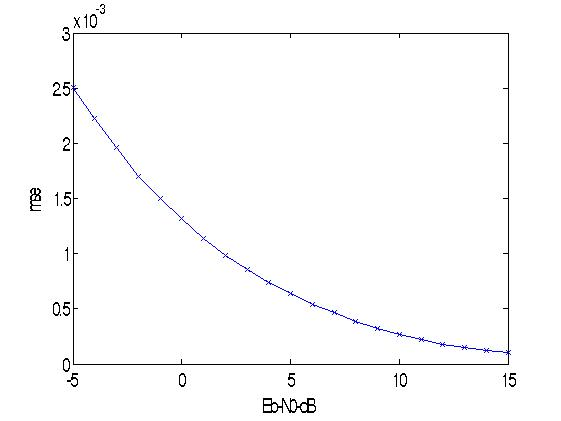
\includegraphics[height = 7 cm]{ebn0bbvsmse.jpg}
\caption{Mse vs SNR for the sensing model, for distributed and centralised solvers}
\label{msevssnr}
\end{figure}

It remains an ongoing task find the discrepancy in the simulation.

\section{Further Work and Project Plan}
Initially, the simulations will be extended to included explicit spatial models. For example, place several simulated base-stations in the square 
\( \left[ 0,1 \right] \times \left[ 0,1 \right] \), at position vectors \(  \{ \textbf{x}_s \}_{s=1}^{N_s} \). 

Given some technical assumptions (\cite{Giannakis2}) - uncorrelated channel taps, and independent, stationary, and memoryless sources -, the spectral density can be written as follows:

\begin{equation}
\Phi_s =\left(f\right) = \sum_{\nu = 1}^{N_b} \theta_{s\nu}b_{\nu}\left(f\right).
\end{equation}
where \(b_{\nu}\) are some suitably chosen bases (for example 2D Gaussians, Splines or rectangle functions), and \(\theta_{i\nu}\) are expansion coefficients to be determined. The PSD at the receivers can be determined as:

\begin{align}
\Phi_r &= \sum_{s=1}^{N_s} \gamma_{sr} \Phi_s \left(f \right) + \sigma_{r}^2 \\
&= \sum_{s=1}^{N_s}\gamma_{sr}\sum_{\nu = 1}^{N_b} \theta_{s\nu}b_{\nu}\left(f\right) +\sigma_{r}^2 \\
&= \textbf{b}_r^T \left(f\right) \vec{ \theta }  + \sigma_{r}^2
\end{align}

This is exactly the kind of convex optimisation problem that can be attacked by the methods described in previous sections (by finding the minimum \(\theta\) and \(\sigma\) pairs which satisfy the measurements.

The end result of this series of simulations should be a 'heat map' showing the locations of the PUs (with heat representing signal strength in decibels). This is a medium risk project - even though the experiments have been done before, setting up and solving the spatial model is quite involved. This work should take me to January at the latest. 

Currently all the data being used to verify the correctness of the algorithms are synthetic. This is a  expedient situation, as currently we do not posses real data. (It also makes debugging the system much easier). By using real data we can get a much better idea of how the system performs, as well as an idea of the real challenges such systems face. 

Investigating the performance on real data would be a medium to high risk endeavour. It depends entirely on the data. Simply providing a noisy PSD would present challenges in terms of the computational load, and a slight re-thinking of the model may be required (this is an unlikely scenario). Detailed spatio-frequency data of central London would require a complete rethink of the approach, as the data would be far too rich for the model provided. Obtaining, cleaning and running the data on the model would take until Christmas, but it could be several months afterwards until definite conclusions could be drawn. 

Current distributed optimisation algorithms (such as D-ADMM) require a colouring of the graph (which acts like a TDMA protocol) to co-ordinate message passing. However, as nodes join the graph, a recolouring is required (else the colouring will end up as \(n\) colours for \(n\) nodes). As colouring a graph is an NP-hard operation, this situation is undesirable. Investigating colouring schemes which may be sub-optimal but nevertheless can add nodes in an ad-hoc manner, but which still preserve the colouring would be one way to avoid the previous situation.

An alternative approach would be to investigate the use of well established graphical algorithms such as belief-propagation (this may require some thinking as to exactly how the coding problem translates to the convex optimisation scenario). Or, see if other graph parameters (or other multiple access schemes) will suffice to 'localise' the algorithm to make the system more flexible. 

Move away from MWC-type measurements at the nodes (e.g. try random demodulators, naive sensing etc)

On the Group Testing front, explicit dependence between items is not currently modelled in the literature. You would expect, however, that defective items would be clustered together (you can imagine that soldiers returning from the same part of the world would have similar incidences of syphilis for example). Also, the source coding models used (Huffman/Shannon-Fano coding) are notoriously inflexible: they require full knowledge of the probabilities 'up-front', and are relatively computationally intensive. It would be desirable to change this. 

One approach to both these problems, would be to investigate the use of the 'succinct' data structure (\cite{Patrescu}), 'Succincter' developed by Mihai Patrescu as a more flexible source coding model (section 4 of (\cite{Patrescu}) describes how to implement arithmetic coding using this structure). How to perform 'pilot' tests, when the items have dependencies is still unclear. This is a high risk piece of work, as it requires some new ideas about how to test items. Previously, the independence of defectives has been leveraged to design testing strategies. It's not as straightforwardly clear what to do when items aren't defective, let alone optimise such a procedure.

We also have a Group Testing algorithm which is a more direct generalisation of Hwang's original algorithm but we have run into difficulties analysing the 'pilot test' part. This is an ongoing project, and will only be worked on as ideas present themselves.

Finally, we have ideas about general strong converses in Group Testing (and sparse inference more generally) that we are exploring. This work is highly ill-defined at present, and as such presents a high-risk. However, it is likely to prove fruitful and can be worked on in conjunction with other projects.